%!TEX root = ../Thesis.tex

\section{Long-Short Term Memory}
\label{sec:Long-Short-Term-Memory}
In the Recurrent Neural Network the internal state $b_h^t$ must be updated in each iteration. This means the effect of some input $x_i^{t_0}$ on $b_h^{t}$, will decay as $t \gg t_0$. This issue is addressed in the Long-Short Term Memory Model (LSTM) by taking inspiration from a computer memory cell.

A computer memory cell can either be written to, read from or reset. On the most basic level memory cell are binary, not just in terms of what can be stored by also in terms of the 3 operations. Either the memory cell is completely reset or not reset, either completely read from or not read from and similarly for writing.

From a mathematical perspective all these operations becomes threshold functions, which are not continuous and therefore not differentiable. This makes them impractical to use in a neural network setting, as neural networks are optimized using gradient descent. The solution is not to use threshold function but a combination of differentiable non-linear activation functions, such as the sigmoid or hyperbolic tangent function.

\subsection{The transistor}

The memory part (cell) of the \textit{memory block} is from a mathematical modeling perspective just a variable. The complexity in the differentiable memory block lies in how that memory is controlled. There are 3 operations read, write and reset. Each of these operations are controlled by a mechanism that resembles a transistor.

\begin{figure}[h]
	\centering
	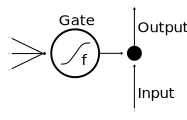
\includegraphics[scale=0.7]{theory/lstm-transistor}
	\caption{Visualization of the differentiable transistor.}
	\label{fig:theory:lstm:lstm-transistor}
\end{figure}

A transistor have an input (\textit{collector}) which is send to the output (\textit{emitter}). In a circuit transistor the output is only equal to the input if the gate (\textit{base}) voltage exceeds a certain threshold, otherwise the output have zero voltage. In the differentiable transistor the idea is the same, except that the gate have a continues value typically in the interval $[0, 1]$. The output value is thus calculated by multiplying the gate value with the input value.
\begin{equation}
a_{output} = b_{gate} a_{input}
\end{equation}

The gate value is typically created from a weighted sum of other values, such as the input vector. To control this sum a non-linear function $f$ is used, typically this is the sigmoid function such that the gate value is in the expected interval $[0, 1]$.
\begin{equation}
b_{gate} = f(a_{gate}), \quad a_{gate} = \sum_{i=1}^I w_i x_i
\end{equation}

\subsection{The memory block}

The LSTM model is the same as the RNN model except that all non-linear units are replaced by a differentiable memory block. The differentiable memory block have an \textit{input} corresponding to $a_{h_\ell}^t$ and an \textit{output} corresponding to $b_{h_\ell}^t$ in the RNN model. To control the three memory operations in the memory block, there are three gates. The \textit{Input Gate} ($b_{\rho_\ell}^t$), \textit{Forget Gate} ($b_{\phi_\ell}$) and \textit{Output Gate} ($b_{\omega_\ell}^t$).

\begin{figure}[h]
	\centering
	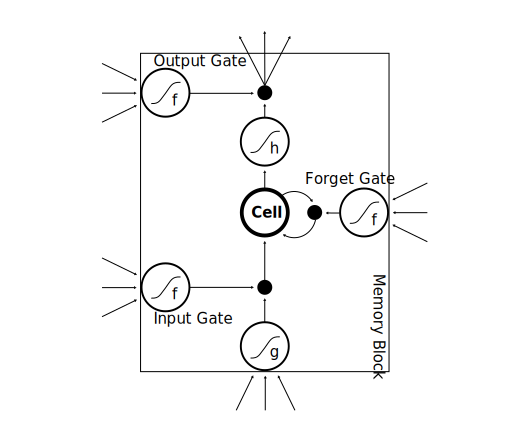
\includegraphics[scale=0.7]{theory/lstm-block}
	\caption{Visualization of the differentiable memory block.}
	\label{fig:theory:lstm:lstm-block}
\end{figure}

Consider Figure \ref{fig:theory:lstm:lstm-block}. The cell state $s_{c_\ell}^t$ is updated as a combination (sum) of the transistor output from the previous \textit{cell} value $s_{c_\ell}^{t-1}$ and the transistor output of the \textit{memory block} input $g(a_{h_\ell}^t)$:
\begin{equation}
s_{c_\ell}^t = b_{\phi_\ell}^t s_{c_\ell}^{t-1} + b_{\rho_\ell}^t g(a_{h_\ell}^t)
\end{equation}

Here $b_{\phi_\ell}^t$ and $b_{\rho_\ell}^t$ are the values of respectively the \textit{forget gate} and \textit{input gate}. Thus if $b_{\phi_\ell}^t = 0$, the cell state is completely forgotten and if $b_{\phi_\ell}^t = 1$ it is fully remembered, however the \textit{memory block} input can still affect its final value. The input part of the cell state update is controlled by the \textit{input gate} $b_{\rho_\ell}^t$. 

The gate values are all calculated using a weighted sum of the input vector $x_i^t$ and previous hidden output $b_{h_\ell}^{t-1}$, just like the $a_{h_\ell}$ value in RNN. This sum is then transformed using a non-linear function $f$, such that the gate value is within $[0, 1]$.
\begin{equation}
\begin{aligned}
a_{\rho_\ell}^t &= \sum_{i=1}^I w_{i, \rho_\ell} x_i^t + \sum_{h'=1}^H w_{h'_\ell, \rho_\ell} b_{h'_\ell}^{t-1} \\
b_{\rho_\ell}^t &= f(a_{\rho_\ell}^t)
\end{aligned}
\label{eq:theory:lstm:gate-value-example}
\end{equation}

Equation \eqref{eq:theory:lstm:gate-value-example} is just for the input gate ($\rho$). The equations for the forget gate ($\phi$) and output gate ($\omega$) are similar, just replace the gate symbol. Note also that while the non-linear function $f$ is the same for all gates, the weights are different.

The memory output is created from the cell state and the output gate:
\begin{equation}
b_{h_\ell}^t = b_{\omega_\ell}^t h(s_{c_\ell}^t)
\end{equation}

$h$ is yet another non-linear function, typically the sigmoid $\sigma(\cdot)$ or hyperbolic tangent $\tanh(\cdot)$ function is used, though it is also normal to simple use the identity function $\theta(a) = a$. An interesting properly of using the identity function is that the LSTM unit generalizes to the simple RNN unit, by setting $b_{\rho_t}^t = 1, b_{\phi_t}^t = 1, b_{\omega_t}^t = 1$

\newpage
\subsection{Forward pass}

\begin{figure}[h]
	\centering
	\centerline{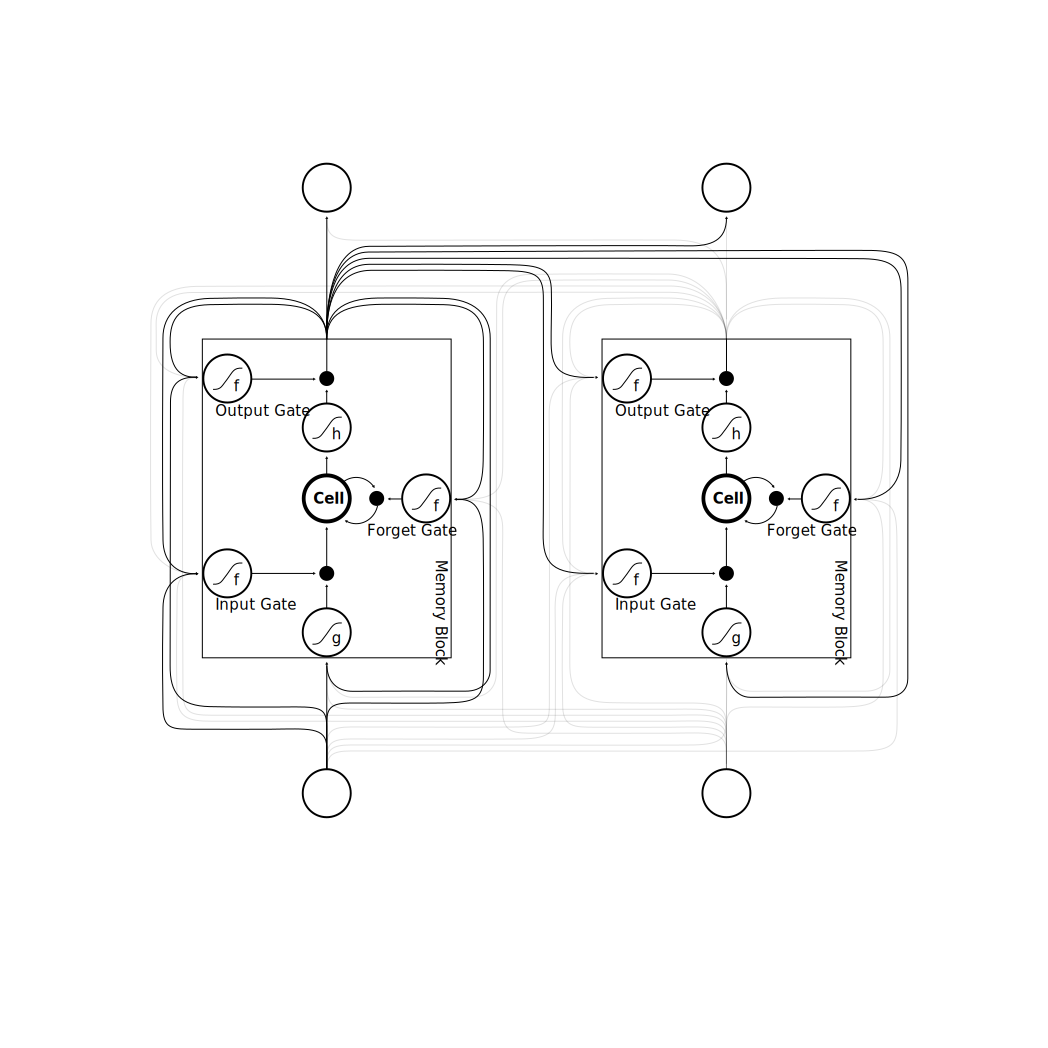
\includegraphics[width=\textwidth]{theory/lstm-network}}
	\caption{Visualization of a LSTM neural network with a single hidden layer.}
	\label{fig:theory:lstm:lstm-network}
\end{figure}

Figure \ref{fig:theory:lstm:lstm-network} shows a very simple LSTM network. It have the recurrent property from the RNN in that the output from the memory blocks are used as input in the next iteration. Figure \ref{fig:theory:lstm:lstm-network} only shows two inputs, but in general there are no restrictions. For simplicity only a single layer is shown, however a multilayer LSTM network can easily be constructed, in the same way a multilayer RNN is constructed. That is by making the output of the memory blocks in the current hidden layer go into the next hidden layer. 

By using the memory block equations and generalizing too $L$ hidden layers, the full set of equations becomes:

\begin{equationbox}[H]
Memory Block Input:
\begin{equation*}
\begin{aligned}
a_{h_\ell}^t &= \sum_{h_{\ell-1}=1}^{H_{\ell-1}} w_{h_{\ell-1}, h_\ell} b_{h_{\ell-1}}^t + \sum_{h'=1}^H w_{h'_\ell, h_\ell} b_{h'_\ell}^{t-1} && \forall \ell \in [1, L] \text{ where: } b_{h_0}^t = x_i^t
\end{aligned}
\end{equation*}
Input Gate:
\begin{equation*}
\begin{aligned}
a_{\rho_\ell}^t &= \sum_{h_{\ell-1}=1}^{H_{\ell-1}} w_{h_{\ell-1}, \rho_\ell} b_{h_{\ell-1}}^t + \sum_{h'=1}^H w_{h'_\ell, \rho_\ell} b_{h'_\ell}^{t-1} && \forall \ell \in [1, L] \text{ where: } b_{h_0}^t = x_i^t \\
b_{\rho_\ell}^t &= f(a_{\rho_\ell}^t) && \forall \ell \in [1, L] 
\end{aligned}
\end{equation*}
Forget Gate:
\begin{equation*}
\begin{aligned}
a_{\phi_\ell}^t &= \sum_{h_{\ell-1}=1}^{H_{\ell-1}} w_{h_{\ell-1}, \phi_\ell} b_{h_{\ell-1}}^t + \sum_{h'=1}^H w_{h'_\ell, \phi_\ell} b_{h'_\ell}^{t-1} && \forall \ell \in [1, L] \text{ where: } b_{h_0}^t = x_i^t\\
b_{\phi_\ell}^t &= f(a_{\phi_\ell}^t) && \forall \ell \in [1, L] 
\end{aligned}
\end{equation*}
Cell State:
\begin{equation*}
\begin{aligned}
s_{c_\ell}^t &= b_{\phi_\ell}^t s_{c_\ell}^{t-1} + b_{\rho_\ell}^t g(a_{h_\ell}^t) && \forall \ell \in [1, L] \text{ where: } c_\ell = \phi_\ell = c_\ell = \rho_\ell
\end{aligned}
\end{equation*}
Output Gate:
\begin{equation*}
\begin{aligned}
a_{\omega_\ell}^t &= \sum_{h_{\ell-1}=1}^{H_{\ell-1}} w_{h_{\ell-1}, \omega_\ell} b_{h_{\ell-1}}^t + \sum_{h'=1}^H w_{h'_\ell, \omega_\ell} b_{h'_\ell}^{t-1} && \forall \ell \in [1, L] \text{ where: } b_{h_0}^t = x_i^t \\
b_{\omega_\ell}^t &= f(a_{\omega_\ell}^t) && \forall \ell \in [1, L] 
\end{aligned}
\end{equation*}
Memory Block Output:
\begin{equation*}
\begin{aligned}
b_{h_\ell}^t &= b_{\omega_\ell}^t h(s_{c_\ell}^t) && \forall \ell \in [1, L] \text{ where: } h_\ell = \omega_\ell = c_\ell
\end{aligned}
\end{equation*}
Network Output:
\begin{equation*}
\begin{aligned}
a_k^t = a_{h_{L+1}}^t &= \sum_{h_L=1}^{H_L} w_{h_L, h_{L+1}} b_{h_L}^t \\
y_k^t &= \frac{\exp(a_k)}{\sum_{k'=1}^K \exp(a_{k'})}
\end{aligned}
\end{equation*}
\caption{Forward equations for a multilayer LSTM network.}
\end{equationbox}

\newpage
\subsection{Backward pass}
\label{sec:theory:lstm:backward-pass}

The backward pass strategy is similar to that used in RNN, except that in the LSTM one have to deal with much more $\delta$ bookkeeping.

The loss function is the same as always:
\begin{equation}
\mathcal{L} = - \sum_{t=1}^T \sum_{k=1}^K t_k^t \ln(y_k^t)
\end{equation}
The starting point is also the same. That is the derivative of the loss function with respect to the first weights. To keep it short the generalization for all layers will be considered immediately.
\begin{equation}
\frac{\partial \mathcal{L}}{\partial w_{h_{\ell-1}, h_\ell}}
= \sum_{t=1}^T \frac{\partial \mathcal{L}}{\partial a_{h_\ell}^t} \frac{\partial a_{h_\ell}^t}{\partial w_{h_{\ell-1}, h_\ell}}
= \sum_{t=1}^T \delta_{h_\ell}^t b_{h_{\ell-1}}^t
\quad \text{where: } \delta_{h_\ell}^t \defeq \frac{\partial \mathcal{L}}{\partial a_{h_\ell}^t}
\end{equation}

From now on there will be some differences. The first is that $a_{h_\ell}^t$ now affects $s_{c_\ell}^t$, thus the equations for $\delta_{h_\ell}^t$ are different:
\begin{equation}
\delta_{h_\ell}^t
= \frac{\partial \mathcal{L}}{\partial a_{h_\ell}^t}
= \frac{\partial \mathcal{L}}{\partial s_{c_\ell}^t} \frac{\partial s_{c_\ell}^t}{\partial a_{h_\ell}^t}
= \epsilon_{s_\ell}^t b_{\rho_\ell}{g'(a_{h_\ell}^t)}
\quad \text{where: } \epsilon_{s_\ell}^t \defeq \frac{\partial \mathcal{L}}{\partial s_{c_\ell}^t}
\end{equation}

Note that a new bookkeeping variable, namely $\epsilon_{s_\ell}^t$ have been introduced. To derive the equations for this value the chain rule is again used. This time it's seen that $\epsilon_{s_\ell}^t$ affects the memory block output $b_{h_\ell}^t$ and itself in the next time iteration $s_{c_\ell}^{t+1}$:
\begin{equation*}
\epsilon_{s_\ell}^t
= \frac{\partial \mathcal{L}}{\partial s_{c_\ell}^t}
= \frac{\partial \mathcal{L}}{\partial b_{h_\ell}^t}\frac{\partial b_{h_\ell}^t}{\partial s_{c_\ell}^t} + \frac{\partial \mathcal{L}}{\partial s_{c_\ell}^{t+1}} \frac{\partial s_{c_\ell}^{t+1}}{\partial s_{c_\ell}^t}
= \epsilon_{b_\ell}^t b_{\omega_\ell}^t h'(s_{c_\ell}^t) + \epsilon_{s_\ell}^{t+1} b_{\phi_\ell}^{t+1}
\quad \text{where: } \epsilon_{b_\ell}^t \defeq \frac{\partial \mathcal{L}}{\partial b_{h_\ell}^t}
\end{equation*}

Again a new bookkeeping variable is introduced. Calculating $\epsilon_{b_\ell}^t$ is quite complicated because $b_{h_\ell}^t$ affects many other parts of the network.

There are two cases, in both cases it affects the current layer on all gates and the memory block input ($a_{h_\ell}^{t+1}, a_{\rho_\ell}^{t+1}, a_{\phi_\ell}^{t+1}, a_{\omega_\ell}^{t+1}$). If the next layer is a hidden layer then it also affects all of its gates and the memory block input ($a_{h_{\ell+1}}^t, a_{\rho_{\ell+1}}^t, a_{\phi_{\ell+1}}^t, a_{\omega_{\ell+1}}^t$). Otherwise if the next layer is not a hidden layer then it affects the network output ($a_k$).

Lets first consider the case where the next layer is a hidden layer ($\ell \in [1, L+1]$), using the chain rule one gets:
\begin{equation}
\begin{aligned}
\epsilon_{b_\ell}^t &=
	\sum_{h'_\ell=1}^{H_\ell} \delta_{h'_\ell}^{t+1} w_{h_\ell, h'_\ell}
	+ \sum_{\rho_\ell=1}^{H_\ell} \delta_{\rho_\ell}^{t+1} w_{h_\ell, \rho_\ell}
	+ \sum_{\phi_\ell=1}^{H_\ell} \delta_{\phi_\ell}^{t+1} w_{h_\ell, \phi_\ell} \\
&+
	 \sum_{\omega_\ell=1}^{H_\ell} \delta_{\omega_\ell}^{t+1} w_{h_\ell, \omega_\ell}
	+ \sum_{h'_{\ell+1}=1}^{H_{\ell+1}} \delta_{h'_{\ell+1}}^t w_{h_\ell, h'_{\ell+1}}
	+ \sum_{\rho_{\ell+1}=1}^{H_{\ell+1}} \delta_{\rho_{\ell+1}}^t w_{h_\ell, \rho_{\ell+1}} \\
&+
	\sum_{\phi_{\ell+1}=1}^{H_{\ell+1}} \delta_{\phi_{\ell+1}}^t w_{h_\ell, \phi_{\ell+1}}
	+ \sum_{\omega_{\ell+1}=1}^{H_{\ell+1}} \delta_{\omega_{\ell+1}}^t w_{h_\ell, \omega_{\ell+1}}
	\quad \forall \ell \in [1, L - 1]
\end{aligned}
\end{equation}

In the other case where the next layer is the output later ($\ell = L$) one gets:
\begin{equation}
\begin{aligned}
\epsilon_{b_L}^t &=
	\sum_{h'_L=1}^{H_L} \delta_{h'_L}^{t+1} w_{h_L, h'_L}
	+ \sum_{\rho_L=1}^{H_L} \delta_{\rho_L}^{t+1} w_{h_L, \rho_L}
	+ \sum_{\phi_L=1}^{H_L} \delta_{\phi_L}^{t+1} w_{h_L, \phi_L} \\
&+
	\sum_{\omega_L=1}^{H_L} \delta_{\omega_L}^{t+1} w_{h_L, \omega_L}
	+ \sum_{k=1}^{K} \delta_{k}^t w_{h_L, k}
\end{aligned}
\end{equation}

This introduces 4 new bookkeeping values:
\begin{equation}
\delta_{\rho_\ell}^t \defeq \frac{\partial \mathcal{L}}{\partial a_{\rho_\ell}}
,\quad \delta_{\phi_\ell}^t \defeq \frac{\partial \mathcal{L}}{\partial a_{\phi_\ell}}
,\quad \delta_{\omega_\ell}^t \defeq \frac{\partial \mathcal{L}}{\partial a_{\omega_\ell}}
,\quad \delta_k^t \defeq \frac{\partial \mathcal{L}}{\partial a_k} 
\end{equation}

Each of these bookkeeping values are a bit different, but the chain rule is still used to derive them. First is $\delta_{\rho_\ell}^t$, through $b_{\rho_\ell}^t$ this affects $s_{c_\ell}^t$.
\begin{equation}
\delta_{\rho_\ell}^t
= \frac{\partial \mathcal{L}}{\partial a_{\rho_\ell}^t}
= \frac{\partial \mathcal{L}}{\partial b_{\rho_\ell}^t} \frac{\partial b_{\rho_\ell}^t}{\partial a_{\rho_\ell}^t}
= \frac{\partial \mathcal{L}}{\partial s_{c_\ell}^t} \frac{\partial s_{c_\ell}^t}{\partial b_{\rho_\ell}^t} \frac{\partial b_{\rho_\ell}^t}{\partial a_{\rho_\ell}^t}
= \epsilon_{s_\ell}^t g(a_{h_\ell}^t) f'(a_{\rho_\ell}^t)
\end{equation}

Next is $\delta_{\phi_\ell}^t$, the situation is somewhat the same, $a_{\phi_\ell}^t$ affects $s_{c_\ell}^t$ through $b_{\phi_\ell}^t$:
\begin{equation}
\delta_{\phi_\ell}^t
= \frac{\partial \mathcal{L}}{\partial a_{\phi_\ell}^t}
= \frac{\partial \mathcal{L}}{\partial b_{\phi_\ell}^t} \frac{\partial b_{\phi_\ell}^t}{\partial a_{\phi_\ell}^t}
= \frac{\partial \mathcal{L}}{\partial s_{c_\ell}^t} \frac{\partial s_{c_\ell}^t}{\partial b_{\phi_\ell}^t} \frac{\partial b_{\phi_\ell}^t}{\partial a_{\phi_\ell}^t}
= \epsilon_{s_\ell}^t s_{c_\ell}^{t-1} f'(a_{\phi_\ell}^t)
\end{equation}

Then $\delta_{\omega_\ell}^t$, here $a_{\omega_\ell}^t$ affects $b_{h_\ell}^t$ through $b_{\omega_\ell}^t$:
\begin{equation}
\delta_{\omega_\ell}^t
= \frac{\partial \mathcal{L}}{\partial a_{\omega_\ell}^t}
= \frac{\partial \mathcal{L}}{\partial b_{\omega_\ell}^t} \frac{\partial b_{\omega_\ell}^t}{\partial a_{\omega_\ell}^t}
= \frac{\partial \mathcal{L}}{\partial b_{h_\ell}^t} \frac{\partial b_{h_\ell}^t}{\partial b_{\omega_\ell}^t} \frac{\partial b_{\omega_\ell}^t}{\partial a_{\omega_\ell}^t}
= \epsilon_{b_\ell}^t h(s_{c_\ell}^t) f'(a_{\omega_\ell}^t)
\end{equation}

Finally there is $\delta_k^t$, here $a_k^t$ affects $y_k^t$. This is no different from the RNN or FFNN case, thus one gets:
\begin{equation}
\delta_k^t = \frac{\partial \mathcal{L}}{\partial y_k^t} \frac{\partial y_k^t}{\partial a_k^t} = y_k^t - t_k^t
\end{equation}

The $\delta$ and $\epsilon$ values can be calculated by going back though the network and by initializing with $\delta_{\rho_\ell}^{T+1} = \delta_{\phi_\ell}^{T+1} = \delta_{\omega_\ell}^{T+1} = \delta_{h_\ell}^{T+1} = \epsilon_{s_\ell}^{T+1} = 0$. 

Until now only $\frac{\partial \mathcal{L}}{\partial w_{h_{\ell-1}, h_\ell}}$ have been considered. But now that $\delta$ and $\epsilon$ values are fully expressed, the remaining derivatives are quite simple.
\begin{align}
\frac{\partial \mathcal{L}}{\partial w_{h'_\ell, h_\ell}}
= \frac{\partial \mathcal{L}}{\partial a_{h_\ell}^t} \frac{\partial a_{h_\ell}^t}{\partial w_{h'_\ell, h_\ell}}
= \delta_{h_\ell}^t b_{h'_\ell}^{t-1}
\end{align}

The gate weights are almost identical:
\begin{align}
\frac{\partial \mathcal{L}}{\partial w_{h_{\ell-1}, \rho_\ell}}
= \delta_{\rho_\ell}^t b_{h_{\ell-1}}^t, \quad
\frac{\partial \mathcal{L}}{\partial w_{h_\ell, \rho_\ell}}
= \delta_{\rho_\ell}^t b_{h_\ell}^{t-1} \\
\frac{\partial \mathcal{L}}{\partial w_{h_{\ell-1}, \phi_\ell}}
= \delta_{\phi_\ell}^t b_{h_{\ell-1}}^t, \quad
\frac{\partial \mathcal{L}}{\partial w_{h_\ell, \phi_\ell}}
= \delta_{\phi_\ell}^t b_{h_\ell}^{t-1} \\
\frac{\partial \mathcal{L}}{\partial w_{h_{\ell-1}, \omega_\ell}}
= \delta_{\omega_\ell}^t b_{h_{\ell-1}}^t, \quad
\frac{\partial \mathcal{L}}{\partial w_{h_\ell, \omega_\ell}}
= \delta_{\omega_\ell}^t b_{h_\ell}^{t-1}
\end{align}
